\documentclass[notes,xcolor=dvipsnames]{beamer}
\usepackage{etex}
\usepackage{pgf}
\usepackage{color}
\definecolor{lblue}{rgb}{0.5,0.5,1}
\usepackage{xspace}
\usepackage{listings}
\usepackage{adjustbox}
\usepackage{spverbatim}
\usepackage{subcaption}
\captionsetup{compatibility=false}
\usepackage{textpos}
\usepackage{etoolbox}
\usepackage{xparse}
\usepackage[shadow , roundedcorners, customcolors, getthemecolors]{dynblocks}

\usepackage{tikz}
\usepackage{tikz-qtree}
\usetikzlibrary{shapes,arrows,positioning,shadows,trees,shadows.blur}
\usepackage{pgfplots}
\usepackage{filecontents}
\usepackage{rotating}
\usepackage{graphicx}
\usepackage[round]{natbib}
\usepackage{booktabs}
% \usepackage{amsmath}
\usepackage{bm}
\usepackage{extarrows}

\mode<presentation>
{
	%\setbeamertemplate{footline}[page number]
	\setbeamertemplate{footline}{%
  \raisebox{2pt}{\makebox[\paperwidth]{\hfill\makebox[20pt]{\textcolor{gray}{\insertframenumber/\inserttotalframenumber}}}}}
  \usetheme{Goettingen}
	%\usecolortheme{dove}
  \setbeamercovered{transparent}
}


\usepackage[english]{babel}
% or whatever

\usepackage[latin1]{inputenc}
% or whatever

\usepackage{times}
\usepackage[T1]{fontenc}
% Or whatever. Note that the encoding and the font should match. If T1
% does not look nice, try deleting the line with the fontenc.

\newcommand{\parspace}{}
%\newcommand{\parspace}{\vspace{-\baselineskip}}
\newcommand{\NN}{\mathbb{N}}
\newcommand{\PP}{\mathbb{P}}
\newcommand{\ZZ}{\mathbb{Z}}
\newcommand{\FF}{\mathbb{F}}           %% for finite fields
\newcommand{\GG}{\mathbb{G}}

\newcommand{\Zrq}{\mathbb{Z}^\ast_q}
\newcommand{\ZN}{\mathbb{Z}_N}

\newcommand{\cA}{\ensuremath{\mathcal{A}}\xspace}
\newcommand{\cB}{\ensuremath{\mathcal{B}}\xspace}
\newcommand{\cC}{\mathcal{C}}
\newcommand{\cD}{\mathcal{D}}
\newcommand{\cE}{\mathcal{E}}
\newcommand{\cF}{\mathcal{F}}
\newcommand{\cG}{\mathcal{G}}
\newcommand{\cH}{\mathcal{H}}
\newcommand{\cI}{\mathcal{I}}
\newcommand{\cK}{\mathcal{K}}
\newcommand{\cL}{\mathcal{L}}
\newcommand{\cM}{\mathcal{M}}
\newcommand{\cO}{\mathcal{O}}
\newcommand{\cP}{\mathcal{P}}
\newcommand{\cQ}{\mathcal{Q}}
\newcommand{\cR}{\mathcal{R}}
\newcommand{\cS}{\mathcal{S}}
\newcommand{\cT}{\mathcal{T}}
\newcommand{\cU}{\mathcal{U}}
\newcommand{\cX}{\mathcal{X}}

\newcommand{\secpar}{\lambda{}}

% assigment, random-choice, etc.
\newcommand{\asgn}{:=}          % assigment \sigma := (a,b,c)
\newcommand{\algout}{\gets}     % algorithm output (sk,pk) <-- KGen(...), hash- and pr-functions too
\newcommand{\ralgout}{\stackrel{R}{\gets}}     % output of random algorithm
\newcommand{\cmp}{=}            % comparison a = b
\newcommand{\rch}{\in_R}        % random choice x \in_R {0,1}^m

\newcommand{\bits}{\{0,1\}}
\newcommand{\rin}{\in_R}
\newcommand{\rinb}{\rin\bits}
\newcommand{\concat}{\!\parallel\!}
%\newcommand{\bitlength}[1]{\lvert{#1}\rvert_{_2}}

\DeclareMathOperator{\ord}{ord}
\DeclareMathOperator{\mymod}{mod}
\newcommand{\MYMOD}[1]{\;(\mymod {#1})}
\DeclareMathOperator{\lcm}{lcm}
\DeclareMathOperator{\dom}{dom}
\newcommand{\legen}[2]{\bigl(\tfrac{#1}{#2}\bigr)}
\newcommand{\jacob}[2]{\bigl(\tfrac{#1}{#2}\bigr)}

\newcommand{\writtenby}[1]{~\mbox{\normalsize\normalfont{(#1)}}}

% new commands
\newcommand{\pwd}{\mathrm{pw}}
\newcommand{\pwdv}{\ensuremath{\mathbf{pw}}}
\newcommand{\msg}{\mathrm{m}}
\newcommand{\mout}{m_{\mathrm{out}}}
\renewcommand{\min}{m_{\mathrm{in}}}
\newcommand{\pake}{\mathrm{PAKE}}
\newcommand{\iencode}{\ensuremath{\mathtt{iEncode}}\xspace}
\newcommand{\idecode}{\ensuremath{\mathtt{iDecode}}\xspace}
\newcommand{\ihme}{\mathrm{IHME}}
\newcommand{\IHME}{\mathtt{IHME}}
\newcommand{\map}{\mathtt{map}}
\newcommand{\mapinv}{\mathtt{mapinv}}
\newcommand{\para}{\mathtt{par}}
\newcommand{\client}{\ensuremath{\mathtt{client}}\xspace}
\newcommand{\server}{\ensuremath{\mathtt{server}}\xspace}
\newcommand{\role}{\mathtt{role}}
\newcommand{\pk}{\ensuremath{\mathtt{pk}}\xspace}
\newcommand{\sk}{\ensuremath{\mathtt{sk}}\xspace}
\newcommand{\Label}{\ensuremath{\mathtt{label}}\xspace}

\newcommand{\comp}{\ensuremath{\mathcal{C}}\xspace}
\newcommand{\round}{\ensuremath{\mathcal{R}}\xspace}
\newcommand{\com}{\ensuremath{\mathcal{E}}\xspace}

\newcommand{\FKV}{$\mathcal{O}$'KV\xspace}
\newcommand{\FBKV}{$\mathcal{O}$'BKV\xspace}
\newcommand{\FSPAKE}{\ensuremath{\mathcal{O}\mathrm{'SPAKE}}\xspace}
\newcommand{\FGMR}{\ensuremath{\mathcal{O}\mathrm{'GMR}}\xspace}

%\newcommand{\mpake}{\mathbb{F}\textnormal{-}\mathrm{PAKE}}
\newcommand{\mpake}{{\ensuremath{\text{O-PAKE}}}\xspace}
\newcommand{\mpakei}{\mathtt{O\text{-}PAKE}}
\newcommand{\D}{\mathcal{D}}
\newcommand{\pgen}{\ensuremath{\mathtt{PGen}}\xspace}
\newcommand{\init}{\ensuremath{\mathtt{init}}\xspace}
\newcommand{\nextm}{\ensuremath{\mathtt{next}}\xspace}
\newcommand{\conf}{\ensuremath{\mathtt{confirm}}\xspace}
\newcommand{\checks}{\ensuremath{\mathtt{check}}\xspace}
\newcommand{\m}{\mathbf{m}}

\newcommand{\sid}{\mathtt{sid}}
\newcommand{\sids}{\pmb{\mathtt{sid}}}
\newcommand{\trans}{\mathtt{trans}}
\newcommand{\NULL}{\mathtt{null}}
\newcommand{\pid}{\mathtt{pid}}
\newcommand{\key}{\ensuremath{\mathtt{k}}\xspace}
\newcommand{\keys}{\ensuremath{\pmb{\mathtt{k}}}\xspace}
\newcommand{\acc}{\mathtt{acc}}
\newcommand{\term}{\mathtt{term}}
\newcommand{\state}{\ensuremath{\mathtt{state}}}
\newcommand{\states}{\pmb{\mathtt{state}}}
\newcommand{\used}{\mathtt{used}}
\newcommand{\send}{\ensuremath{\mathsf{Send}}\xspace}
\newcommand{\execute}{\ensuremath{\mathsf{Execute}}\xspace}
\newcommand{\reveal}{\ensuremath{\mathsf{Reveal}}\xspace}
\newcommand{\test}{\ensuremath{\mathsf{Test}}\xspace}
\newcommand{\corrupt}{\ensuremath{\mathsf{Corrupt}}\xspace}
\newcommand{\create}{\ensuremath{\mathtt{Create}}\xspace}
\newcommand{\INIT}{\ensuremath{\mathsf{Init}}\xspace}

\newcommand{\MYIF}{\mathtt{If}}
\newcommand{\MYELSE}{\mathtt{Else}}
\newcommand{\MYTHEN}{\mathsf{Then}}

\newcommand{\advo}{\cA_1(\secpar)}
\newcommand{\advt}{\cA_2(\secpar)}

\newcommand{\true}{\mathtt{true}}
\newcommand{\Adv}{\mathsf{Adv}}
\newcommand{\Succ}{\mathsf{Succ}}
\newcommand{\prob}{\ensuremath{\mathrm{Pr}}\xspace}
\newcommand{\Exp}{\ensuremath{\mathsf{Exp}}\xspace}
\newcommand{\Expi}[1]{\ensuremath{\mathsf{Exp}_{#1}}\xspace}
\newcommand{\Expbm}[1]{\ensuremath{\bm{\mathsf{Exp}_{#1}}}\xspace}
\newcommand{\ake}{\mathsf{AKE\text{-}Sec}}
\newcommand{\AKE}{\mathsf{AKE}}
\newcommand{\ROR}{\mathrm{ROR}}
\newcommand{\FTG}{\mathrm{FTG}}
\newcommand{\cauth}{\mathsf{CAuth}}
\newcommand{\sauth}{\mathsf{SAuth}}
\newcommand{\pwhide}{\mathsf{PW\text{-}Hid}}
\newcommand{\npwhide}{n\mathsf{\text{-}PW\text{-}Hid}}
\newcommand{\akefull}{\mathsf{AKE\text{-}FSec}}
\newcommand{\akecpa}{\mathsf{AKE\text{-}CPWA}}
\newcommand{\simul}{\mathsf{Sim}}
\newcommand{\Sim}{\ensuremath{\mathsf{Sim}}\xspace}
\newcommand{\ext}{\mathsf{Ext}}
\newcommand{\calls}{\textnormal{ calls }}
\newcommand{\refalgo}[2]{Algorithm \ref{#1}, Line \ref{#2}}
\newcommand{\refline}[1]{Line \ref{#1}}
\newcommand{\ihide}{\mathsf{ihide}}
\newcommand{\dlin}{\ensuremath{\mathsf{DLIN}}}
\newcommand{\genbg}{{\ensuremath{\mathsf{GenBG}}}}
\newcommand{\cca}{\ensuremath{\mathsf{CCA}}\xspace}
\newcommand{\St}{\mathtt{St}}

\newcommand{\KDF}{\ensuremath{\mathtt{KDF}}\xspace}
\newcommand{\PRF}{\ensuremath{\mathrm{PRF}}\xspace}
\newcommand{\prf}{\ensuremath{\mathtt{prf}}\xspace}
\newcommand{\Enc}{\ensuremath{\mathtt{Enc}}\xspace}
\newcommand{\Dec}{\ensuremath{\mathtt{Dec}}\xspace}
\newcommand{\Gen}{\ensuremath{\mathtt{Gen}}\xspace}
\newcommand{\Mac}{\ensuremath{\mathtt{MAC}}\xspace}

\newcommand{\tbf}[1]{\\\textbf{#1}}

\newcommand{\myhref}[2]{\href{#1}{#2}\footnote{\url{#1}}}

\newcommand{\naive}{na{\"i}ve\xspace}

\newcommand{\myparagraph}[1]{\paragraph{#1.}}
\newcommand{\mysubsubsection}[1]{\subsubsection{#1.}}

\newcommand{\TabEQ}{%
       \setlength{\abovedisplayskip}{-\topskip}%
       \setlength{\belowdisplayskip}{-\topskip}%
}

\newlength{\arrow}
\settowidth{\arrow}{\scriptsize$10000000000000000$}
\newcommand*{\myrightarrow}[1]{\xrightarrow{\mathmakebox[\arrow]{#1}}}
\newcommand*{\myleftarrow}[1]{\xleftarrow{\mathmakebox[\arrow]{#1}}}
\newcommand*{\myleftrightarrow}[1]{\xleftrightarrow{\mathmakebox[\arrow]{#1}}}

\newlength{\shortarrow}
\settowidth{\shortarrow}{\scriptsize$1000000$}
\newcommand*{\myshortrightarrow}[1]{\xrightarrow{\mathmakebox[\shortarrow]{#1}}}
\newcommand*{\myshortleftarrow}[1]{\xleftarrow{\mathmakebox[\shortarrow]{#1}}}
\newcommand*{\myshortleftrightarrow}[1]{\xleftrightarrow{\mathmakebox[\shortarrow]{#1}}}

\newcommand{\marked}[2]{{\color{red}}#2}

\title[Password-based Cryptography] % (optional, use only with long paper titles)
{Advancments in Password-based Cryptography}

\author[F. Kiefer] % (optional, use only with lots of authors)
{Franziskus Kiefer}
% - Give the names in the same order as the appear in the paper.
% - Use the \inst{?} command only if the authors have different
%   affiliation.

\institute[University of Surrey] % (optional, but mostly needed)
{
 Department of Computing Science\\
 University of Surrey
}
% - Use the \inst command only if there are several affiliations.
% - Keep it simple, no one is interested in your street address.

\date[Viva] % (optional, should be abbreviation of conference name)
{PhD Viva}
% - Either use conference name or its abbreviation.
% - Not really informative to the audience, more for people (including
%   yourself) who are reading the slides online

\subject{Password Based Authenticated Key Exchange, PAKE}
% This is only inserted into the PDF information catalog. Can be left
% out. 



% If you have a file called "university-logo-filename.xxx", where xxx
% is a graphic format that can be processed by latex or pdflatex,
% resp., then you can add a logo as follows:

\pgfdeclareimage[height=0.5cm]{university-logo}{University-of-Surrey-logo.jpg}
\logo{\pgfuseimage{university-logo}}



% Delete this, if you do not want the table of contents to pop up at
% the beginning of each subsection:
%\AtBeginSubsection[]
%{
%  \begin{frame}<beamer>{Outline}
%    \tableofcontents[currentsection,currentsubsection]
%  \end{frame}
%}


% If you wish to uncover everything in a step-wise fashion, uncomment
% the following command: 

%\beamerdefaultoverlayspecification{<+->}


\begin{document}

 \tikzset{
    %Define standard arrow tip
    >=stealth',
    %Define style for boxes
    party/.style={
           rectangle,
           rounded corners,
           draw=black, very thick,
           text width=6.5em,
           minimum height=2em,
           text centered},
    state/.style={
           inner sep=0,
           minimum size=0cm},
    box/.style={draw=none,shade,
      top color=blue!40,
      bottom color=blue!5,
      rounded corners=6pt,
      blur shadow={shadow blur steps=5},
      text width=6em},
    bigbox/.style={draw=none,shade,
      top color=blue!40,
      bottom color=blue!5,
      rounded corners=6pt,
      blur shadow={shadow blur steps=5},
      text width=2em,
      minimum height=12em},
    % Define arrow style
    pil/.style={
           ->,
           thick,
           shorten <=2pt,
           shorten >=2pt,},
    circle dotted/.style={dash pattern=on .05mm off 2mm, line cap=round}
}

\begin{frame}
  \titlepage
\end{frame}

\begin{frame}{Outline}
  \tableofcontents %[pausesections]
  % You might wish to add the option [pausesections]
\end{frame}


\section{Introduction \& Motivation}

\subsection{Authentication and Key Exchange}

\begin{frame}{How to Communicate Securely? (1/2)}

	How can I communicate securely with a website?
	
	\vspace*{2em}
	\setbeamercolor{uppercol}{fg=white,bg=blue}%
	\setbeamercolor{lowercol}{fg=black,bg=lblue}%
	\begin{beamerboxesrounded}[upper=uppercol,lower=lowercol,shadow=true]{\centering TLS}\centering
		TLS and HTTPS 
	\end{beamerboxesrounded}

	\vspace*{2em}
  How to securely communicate individualised content from a website?

	\vspace*{2em}
	\setbeamercolor{uppercol}{fg=white,bg=blue}%
	\setbeamercolor{lowercol}{fg=black,bg=lblue}%
	\begin{beamerboxesrounded}[upper=uppercol,lower=lowercol,shadow=true]{\centering Passwords}\centering
		Password over HTML
	\end{beamerboxesrounded}
\end{frame}
	
\begin{frame}{How to Communicate Securely? (2/2)}

\begin{itemize}
	\item Password over HTML is insufficient for authentication
	\item How can two (or more) parties want to communicate securely?
\end{itemize}
	
% 	\vspace*{2em}
% 	\structure{Secure}
% 	\begin{itemize}
% 		\item Authentic
% 		\item Confidential
% 	\end{itemize}

  \pause
	\vspace*{2em}
	\structure{Authenticated Key-Establishement} 
	\begin{itemize}
		\item Key Transport/Distribution
		\item<1-| alert@2> Key Exchange/Agreement
	\end{itemize}
\end{frame}
	
\begin{frame}{Authenticated Key Exchange}

\begin{figure}
\centering
\begin{tikzpicture}
	\node[state,align=center] (client) at (0,0.25) {\pgfimage[width=0.8cm]{os_tux}\\\alert{s}};
	
	\node[state, align=left] (clientText) at (0,-1) {accept $k$};
	\node[state] (client1) at (2,-1){};
	
	\node[state, align=left] at (0,-2) {};
	\node[state] (client2) at (2,-2){};	
	
	
	\node[state,align=center] (server) at (6,0.25) {\pgfimage[width=0.8cm]{techie_sailor}\\\alert{s}};
	
	\node[state, align=right] (serverText) at (6,-1) {accept $k$};
	\node[state] (server1) at (4,-1) {};
	
	\node[state, align=right] at (6,-2) {};
	\node[state] (server2) at (4,-2) {};
	
	\node[cylinder, blue, draw,minimum height=1.5cm, minimum width=1.5cm,aspect=.5, inner xsep=1.5cm, inner ysep=0.5cm] at (2.9,-2) {};
	\draw[pil,<->] (client1) -- node[above] {Key Exchange} (server1);
	\draw[pil,<->] (server2) -- node[above] {Secure Channel} (client2);
	
	\draw[pil,->] (clientText.west) |- (1.5,-2);
	\draw[pil,->] (serverText.east) |- (4.5,-2);
\end{tikzpicture}
%\caption{Encrypted Key Exchange (EKE)}
\label{fig:ke}
\end{figure}

\structure{Authenticated} Key Exchange
\begin{itemize}
	\item Requires \alert{(common) secret}
\end{itemize}

\end{frame}

\subsection{Password Authenticated Key Exchange}

% \begin{frame}{Password Authenticated Key Exchange}{PAKE 1/2}
% 	\begin{quote}
% 	``Humans are incapable of securely storing high-quality cryptographic keys, and they have unacceptable speed and accuracy when performing cryptographic operations.''~\cite{Kaufmann02}
% 	\end{quote}
% 	
% 	\vspace*{2em}
% 	\setbeamercolor{uppercol}{fg=white,bg=blue}%
% 	\setbeamercolor{lowercol}{fg=black,bg=lblue}%
% 	\begin{beamerboxesrounded}[upper=uppercol,lower=lowercol,shadow=true]{\centering Passwords}\centering
% 		Common secret with low entropy
% 	\end{beamerboxesrounded}
% 	
% \end{frame}
%
\begin{frame}{Password Authenticated Key Exchange}{PAKE (s $:=$ password)}
	Inherent threat of dictionary attacks
	\begin{itemize}
		\item Can not prevent online dicionary attacks
		\item PAKE Security:\\\begin{center} \alert{security against offline dictionary attacks}\end{center}
	\end{itemize}
	
	\vspace*{2em}
	Established security models
	\begin{itemize}
		\item Game Based Security Model by \cite{Bellare2000}%[BPR 2001]
		\item Universally Composable PAKE by \cite{Canetti2005}%[CHKLK 2005]
	\end{itemize}
%	Well established research area since 2000
%	\begin{itemize}
%		\item Simple password-based encrypted key exchange protocols by \cite{Abdalla2005}
%		\item Faster and shorter password-authenticated key exchange by \cite{Gennaro2008}
%		\item Round-Optimal Password-Based Authenticated Key Exchange by \cite{Katz2011}
%		\item \dots
%	\end{itemize}
\end{frame}

\begin{frame}{Password Authenticated Key Exchange}{SPAKE}

 \cite{Abdalla2005}: SPAKE uses DL-hard group $G$ and public $M,N\in G$; hash function $H$ as random oracle

\begin{figure}
\centering
\begin{tikzpicture}
	\node[state] (client) at (0,0.25) {\pgfimage[width=0.8cm]{os_tux}};
	
	\node[state, align=left] at (0,-1) {$x\rin\ZZ_p, X\gets g^x$\\  $\color{red} X'\gets X\cdot M^\pwd$};
	\node[state] (client1) at (2,-1){};
	
	\node[state, align=left] at (0,-2) {$K'_A\gets {\color{red} (Y'/N^\pwd)}^x$};
	\node[state] (client2) at (2,-2){};	
	
	%\node[state, align=center] at (0,-3) {$K\gets H(A,B,X',Y',K_A,\pwd)$};
	
	
	\node[state] (server) at (6,0.25) {\pgfimage[width=0.8cm]{techie_sailor}};
	
	\node[state, align=right] at (6,-1) {$y\rin\ZZ_p, Y\gets g^y$\\ $\color{red} Y'\gets Y\cdot N^\pwd$};
	\node[state] (server1) at (4,-1) {};
	
	\node[state, align=right] at (6,-2) {$K'_B\gets {\color{red} (X'/M^\pwd)}^y$};
	\node[state] (server2) at (4,-2) {};
	
	%\node[state, align=center] at (6,-3) {$K\gets H(A,B,X',Y',K_B,\pwd)$};
	
	\draw[pil] (client1) -- node[above] {$X'$} (server1);
	\draw[pil] (server2) -- node[above] {$Y'$} (client2);
\end{tikzpicture}
\label{fig:eke}
\end{figure}
Key derivation:\\
$K_A\gets H(A,B,X',Y',K'_A,\pwd)$\\
$K_B\gets H(A,B,X',Y',K'_B,\pwd)$

\end{frame}

\subsection{PAKE Security Models}

\begin{frame}{PAKE Security Model 1/2}{Authenticated Key Exchange (AKE) 1/2}
The PPT adversary $\mathcal{A}$ has access to the following oracles:
\begin{description}
    \item[$m'\gets\mathsf{Send}(P,P',m)$:] \hfill \\ simulates active attack.
    \item[$\mathtt{t}\gets\mathsf{Execute}(P,P')$:] \hfill \\ simulates passive attack
    \item[$\pwd\gets\mathsf{Corrupt}(P, P')$:] \hfill \\ simulates password leakage
    \item[$\mathtt{k}_\mathcal{A}\gets\mathsf{Test}(P)$:] \hfill \\ returns real or random key (security definition)
\end{description}
\end{frame}

\begin{frame}{PAKE Security Model 1/2}{Authenticated Key Exchange (AKE) 2/2}
\begin{definition}[AKE-Security]\label{def:ake}
A PAKE protocol $\Pi$ is \emph{AKE-secure} if for all dictionaries $\mathcal{D}$ and for all PPT adversaries $\mathcal{A}$ using at most $t$ active attacks there exists a negligible function $\varepsilon(\cdot)$ such that:
\[\left|\Pr[\mathsf{Exp}_{\Pi,\mathcal{A}}^{\mathsf{AKE-SEC}}(\lambda)=1]-\frac12\right|\leq \frac{\mathcal{O}(t)}{|\mathcal{D}|}+\varepsilon(\lambda).\]

\noindent$\mathsf{Exp}_{\Pi,\mathcal{A}}^{\mathsf{AKE-SEC}}(\lambda):$ \\
\hspace*{2em} $b\in_R\{0,1\}$\\
\hspace*{2em} $b'\gets\mathcal{A}^{\mathsf{Send},\mathsf{Execute},\mathsf{Corrupt},\mathsf{Test}}(\lambda)$\\
\hspace*{2em} return $b=b'$
\end{definition}
$\mathsf{Test}$ may only be asked on \emph{fresh} session.
\end{frame}

\begin{frame}{PAKE Security Model 2/2}{Universal Composability (UC) 1/2}
The following entities are involved:
\begin{description}
    \item[$\mathcal{Z}$:] \hfill \\ environment/distinguisher
    \item[$\Pi$:] \hfill \\ a real-world PAKE protocol
    \item[$\mathcal{A}$:] \hfill \\ real-world adversary on $\Pi$
    \item[$\mathcal{F}_{\text{PAKE}}$:] \hfill \\ ideal functionality for PAKE protocols
    \item[$\mathcal{S}$:] \hfill \\ ideal-world adversary
\end{description}
\end{frame}

\begin{frame}{PAKE Security Model 2/2}{Universal Composability (UC) 2/2}
\begin{definition}[UC-Security]\label{def:uc}
A PAKE protocol $\Pi$ is \emph{UC-secure} if distinguisher $\mathcal{Z}$ is not able to decide whether it is interacting with the real world protocol $\Pi$ and the real world adversary $\mathcal{A}$ or the ideal functionality $\mathcal{F}$ and ideal-world adversary $\mathcal{S}$.
\end{definition}

\end{frame}

% \begin{frame}{Forward-Secrecy in PAKE 1/4}{}
%
% 	Forward-Secrecy is modelled with corruptions
% 	\begin{itemize}
% 		\item Forward-Secrecy: session key will not be compromised if long-term key is compromised in the future
% 		\item Corrupt oracle returns long-term secret (password)
% 	\end{itemize}
%
% \end{frame}
%
% \begin{frame}{Forward-Secrecy in PAKE 2/4}{Corruption Models}
%
% 	\begin{description}
% 		\item[Zero] \hfill \\ $\mathcal{A}$ has no access to the $\mathsf{Corrupt}$ oracle.
% 		\item[Static] \hfill \\ $\mathcal{A}$ has no access to the $\mathsf{Corrupt}$ oracle but can initially retrieve passwords before the experiment starts.
% 		\item[Adaptive] \hfill \\ $\mathcal{A}$ has access to the $\mathsf{Corrupt}(C,S)$ oracle to retrieve $\pwd_{(C,S)}$.
% 		\item[Strong] \hfill \\  $\mathcal{A}$ has access to the $\mathsf{Corrupt}(C,S)$ oracle to retrieve state information of all client instances $C_i$ that have been invoked with server $S$, including $\pwd_{C,S}$.
% 	\end{description}
%
% \end{frame}
%
% \begin{frame}{Forward-Secrecy in PAKE 3/4}{}
%
% 	\begin{dynblock}
% 		First block
% 		\opaqueblock<1>{
% 				\begin{quote}
% 					``The set of malicious users did not need to be considered in the 2-party due to the independence among the passwords shared between pairs of honest participants and those shared with malicious users.''
% 				\end{quote}
% 				\vskip5mm
% 			  \hspace*\fill{\small--- \cite{Abdalla2005a}}
% 		}
% 		\invblock<2->
%
% 		Second block
% 		\opaqueblock<2>{
% 				\begin{quote}
% 					``In the password-only setting, this [static corruption] actually makes no difference because the adversary can internally simulate these oracles by itself.''
% 				\end{quote}
% 				\vskip5mm
% 			  \hspace*\fill{\small--- \cite{Gennaro2008}}
% 		}
% 		\invblock<3->
%
% 		Third block
% 		\opaqueblock<3>{
% 				\begin{quote}
% 					``[...] we consider the original BPR2000 model without [dynamic] Corrupt query because the basic notion of BPR2000 freshness restricts the adversary [...] from corrupting anyone in the model (i.e., effectively restricting $\mathcal{A}$ from asking any Corrupt query).''
% 				\end{quote}
% 				\vskip5mm
% 			  \hspace*\fill{\small--- \cite{ChooBH05}}
% 		}
% 	\end{dynblock}
%
% \end{frame}
%
% \begin{frame}{Forward-Secrecy in PAKE 4/4}{}
%
% 	However
% 	\begin{itemize}
% 		\item No proof for equality of static/adaptive and zero corruption model given
% 		\item No counterexample in the two-party setting exists
% 	\end{itemize}
% 	
% 	\vspace*{2em}
% 	\structure{Contribution}
% 	\begin{itemize}
% 		\item Consolidation of corruption models
% 		\item Impossibility of secure PAKE in the strong corruption model
% 		\item Unfortunately, no proof for equality of adaptive and zero corruption model found (yet)
% 	\end{itemize}
%
% \end{frame}

%===============================================================================
% A Password Authentication Framework for the Single-Server Setting
%===============================================================================

\section{Single-Server Password Framework}%{A Password Authentication Framework for the Single-Server Setting}

\begin{frame}{Table of Content}
\tableofcontents[currentsection]
\end{frame}

\newsavebox{\savelisting}
\newenvironment{listing}
{\vspace*{-2em}\begin{lrbox}{\savelisting}
\begin{minipage}{4.8in}
\begin{flushleft}}
{\end{flushleft}
\end{minipage}
\end{lrbox}
\begin{center}
\resizebox{\columnwidth}{!}{\setlength\fboxsep{6pt}\fbox{\usebox{\savelisting}}}
\end{center}}

\begin{frame}{Password Registration}{Motivation}
  \begin{itemize}
    \item Don't trust servers
    \begin{itemize}
      \item ... to handle passwords properly
    \end{itemize}
    \vspace*{2em}\pause
    \item Don't trust clients
    \begin{itemize}
      \item ... to choose secure passwords
    \end{itemize}
  \end{itemize}
\end{frame}

\begin{frame}{Single-Server Password Authentication Framework}
  \begin{figure}
  \centering
  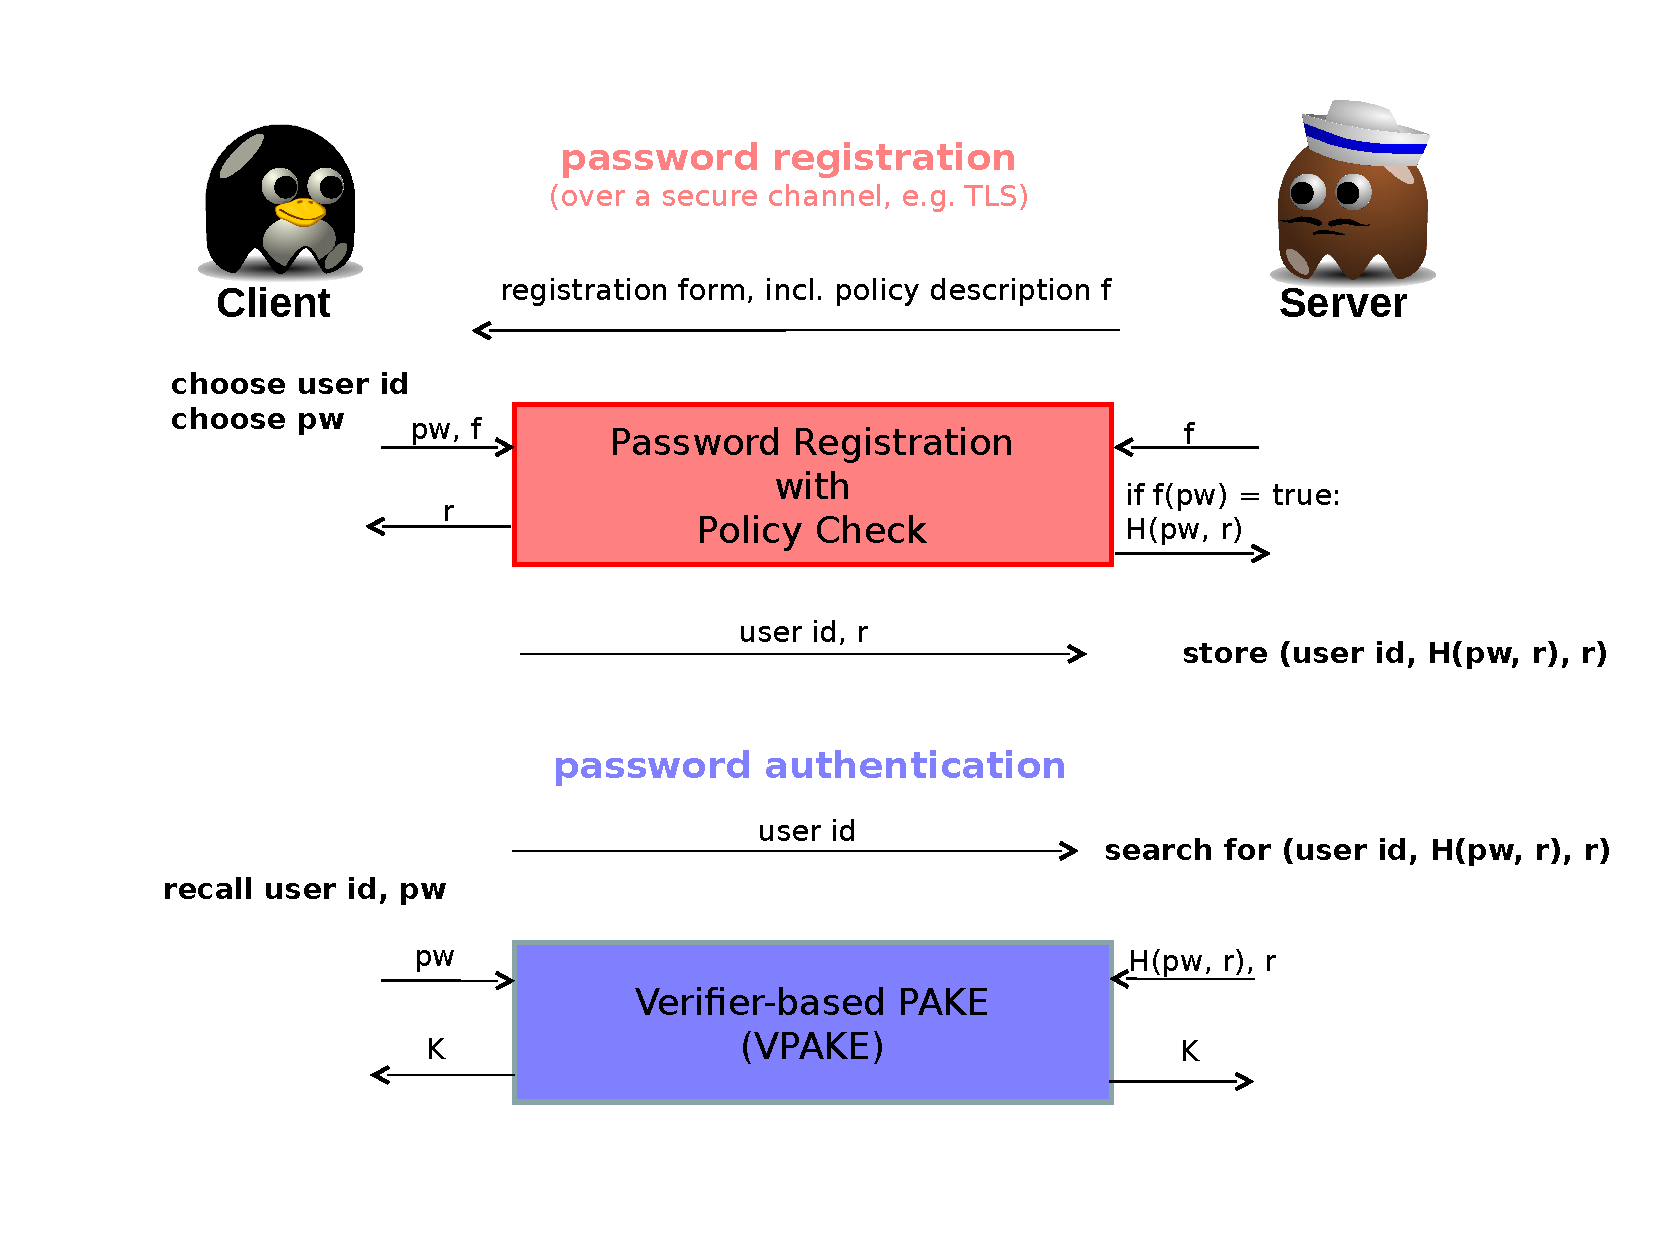
\includegraphics[width=\textwidth]{framework1.pdf}
  \end{figure}
\end{frame}

\subsection{Modelling Password Policies}

\begin{frame}{Passwords}
  
\structure{Password definition}
\begin{itemize}
  \item Using 94 printable ASCII characters ($\Sigma=d\cup u \cup l \cup s$) with four sets
  \begin{itemize}
    \item digits ($d$)
    \item upper case characters ($u$)
    \item lower case characters ($l$)
    \item symbols ($s$)
  \end{itemize}
  \item password is defined as $\pwd=c_1 || \cdots || c_n\in\Sigma^n$
\end{itemize}

\structure{Password Mapping}
\begin{itemize}
  \item $\pi$ denotes integer mapped from $\pwd$
  \item $\pi=\sum_{i=1}^n b^{i-1}p(c_i)$
  \begin{itemize}
    \item $p(c_i)=\texttt{ASCII}(c_i)-32$
    \item $b$ is shift base
  \end{itemize}
  \item $\pi_i$ denotes the encoded i-th character in $\pwd$
\end{itemize}

\end{frame}

\begin{frame}{Password Policies}
  \structure{Policy:} $f=(R, \pmin, \pmax)$
  \begin{itemize}
    \item $R$: policy expression of admissible characters
    \item $\pmin$: minimum number of characters
    \item $\pmax$: maximum number of characters (can be ommited)
  \end{itemize}
  
  \vspace*{2em}
  $f(\pwd)=f(\pi)=\true$ iff:
  \begin{itemize}
    \item $\pwd$ satisfies $R$
    \item $\pmin\leq |\pwd| \leq \pmax$
  \end{itemize}
\end{frame}

\begin{frame}{Password Hashing}
  extended definition from \cite{BenhamoudaP13} (added $s_P$)
%   \begin{tabular}{ll}
%     \structure{PSetup($\lambda$):} & \\
%     & outputs hashing parameters $p$ \\
%     \structure{PPHSalt($p$):} & \\
%     & generates random pre-hash salt $s_P$ \\
%     \structure{PPreHash($p, \pwd, s_P$):} & \\
%     & computes a pre-hash value $P$ \\
%     \structure{PHSalt($p$):} & \\
%     & generates random hashing salt $s_H$ \\
%     \structure{PHash($p, P, s_P, s_H$):} & \\
%     & computes a (final) hash value $H$ \\
%   \end{tabular}
  \begin{description}
    \item[\PSetup($\lambda$):] \hfill\\ outputs hashing parameters $p$
    \item[\PPHSalt($p$):] \hfill\\	generates random pre-hash salt $s_P$
    \item[\PPreHash($p, \pwd, s_P$):] \hfill\\	computes a pre-hash value $P$
    \item[\PHSalt($p$):] \hfill\\ generates random hashing salt $s_H$
    \item[\PHash($p, P, s_P, s_H$):]	\hfill\\ computes a (final) hash value $H$
  \end{description}
  Let $H\gets\mathtt{Hash}(\pwd, s_P, s_H)=\text{PHash}(p, P, s_P, s_H)$ with $P\gets\text{PPreHash}(p, \pwd, s_P)$
\end{frame}

\subsection[ZKPPC]{Zero-Knowledge Password Policy Checks}

% \begin{frame}{Zero-Knowledge Password Policy Checks 1/2}
%   
%   \begin{definition}[Set Membership Proof of Commitment]\label{def:smp}
%   \Com is a commitment scheme, $L$ a set
%   \[
%     \mathtt{ZKPoK}\{(c, r): C\gets\Com(c, r) \wedge c\in L\}
%   \]
%   \end{definition}
%   
%   \begin{definition}[Zero-Knowledge Password Policy Check]\label{def:zkppc}
%   For password hashing scheme $H$, policy $f$, and password $\pi$ ZKPPC is defined as
%   \[
%     \mathtt{ZKPoK}\{(\pi, r): f(\pi)=\true \wedge H\gets\PHash(\pi, r)\}
%   \]
%   \end{definition}
% \end{frame}

\begin{frame}{The ZKPPC Framework}

% \begin{figure}[t]
% \begin{center}
% \scalebox{0.7}{\small
% \begin{tabular}{ l c l }
% \toprule
% {\bf Client} & & {\bf Server} \\
% Input: $(R, n,m), p, C_p$ & & Input: $(R, n, m), p, C_p$ \\
% \midrule
% Choose $\pwd\in_R D_f$ & & \\
% with $f(\pwd)=\true$ & & \\
% Let $n \gets |\pwd|$ & & \\
% for $i\in[0,n-1]$ & & \\
% \hspace*{1em} let $c_i\in\pwd$ & & \\
% \hspace*{1em} $\pi_i\gets\mathtt{chr2int}(c_i, i)$ & & \\
% \hspace*{1em} $r_i\rin\mathbb{S}_C; C_i\gets\mathtt{Com}(\pi_i;r_i)$ & & \\
% $\pi\gets\sum_i\pi_i$; $r\gets\sum_ir_i$ & & \\
% $C\gets\prod_{i}C_i$ & & \\
% $s_P\gets_R\mathtt{PPHSalt}(p)$ & & \\
% $s_H\gets_R\mathtt{PHSalt}(p)$ & $H,~\{C_i\}$ & \\
% $H\gets \mathtt{Hash}(\pi;(s_P, s_H))$ & $\xrightarrow{\makebox[4cm]{$\forall i:~\mathtt{SMP}(\pi_i,r_i,\Omega')$}}$ & Let $n\gets|\{C_i\}|$ \\
%  & & If $n \not\in[n,m]$ then ABORT\\
%  & $\mathtt{ZKPoK}\{(\pi, s_P, s_H, r):$ & Else $C\gets\prod_{i}C_i$ \\
%  & $H=\mathtt{Hash}(\pi; (s_P, s_H))$ & \\
%  & $\xrightarrow{\makebox[4cm]{$\wedge ~ C=\mathtt{Com}(\pi;r)\}$}}$ & If any $\mathtt{SMP}$ or $\mathtt{ZKPoK}$ is\\
%  & & not successful then ABORT \\
%  & & Else ACCEPT and store $H$\\
% \bottomrule
% \end{tabular}
% }
% \end{center}
% % \caption{ZKPPC Framework for ASCII-based Passwords}
% % \label{fig:zkpconeserver}
% \end{figure}

\begin{figure}[t]
\begin{center}
\scalebox{0.7}{\small
\begin{tabular}{ l c l }
\toprule
{\bf Client \Client} & & {\bf Server \Server} \\
Input: $(R,\pmin,\pmax),\paramP,\paramC$ & & Input: $(R,\pmin,\pmax),\paramP,\paramC$ \\
\midrule
Choose $\pwd\in_R\cD_f$ & & \\
with $f(\pwd)=\true$ & & \\
Let $n \gets |\pwd|$ & & \\
for $i\in[0,n-1]$ & & \\
\hspace*{1em} let $c_i\in\pwd$ & & \\
\hspace*{1em} $\pi_i\gets\ichrint(c_i, i)$ & & \\
\hspace*{1em} $r_i\rin\SSS_C; C_i\gets\Com(\pi_i;r_i)$ & & \\
$\pi\gets\sum_i\pi_i$; $r\gets\sum_ir_i$ & & \\
$C\gets\prod_{i}C_i$ & & \\
$s_P\gets_R\PPHSalt(\paramP)$ & & \\
$s_H\gets_R\PHSalt(\paramP)$ & $H,~\{C_i\}$ & \\
$H\gets \HashP(\pi;(s_P, s_H))$ & $\xrightarrow{\makebox[4cm]{$\forall i:~\SMP(\pi_i,r_i,\Omega')$}}$ & Let $n\gets|\{C_i\}|$ \\
 & & If $n \not\in[\pmin,\pmax]$ then ABORT\\
 & $\ZKPoK\{(\pi, s_P, s_H, r):$ & Else $C\gets\prod_{i}C_i$ \\
 & $H=\HashP(\pi; (s_P, s_H))$ & \\
 & $\xrightarrow{\makebox[4cm]{$\wedge ~ C=\Com(\pi;r)\}$}}$ & If any $\SMP$ or $\ZKPoK$ is\\
 & & not successful then ABORT \\
 & & Else ACCEPT and store $H$\\
\bottomrule
\end{tabular}
}
\end{center}
\end{figure}

\end{frame}

\begin{frame}{Zero-Knowledge Password Policy Checks}
  
  Committed ZKPPC
  \begin{align*}    
    \mathtt{ZKPoK}\{(\pi, r, \{r_i\}_{[1,n]}): & C_i=\mathtt{Com}(\pi_i, r_i) ~ \wedge \\
    & \pi_i\in\Omega_j ~ \wedge \\
    & \prod_i^n C_i=\mathtt{Com}(\pi, \sum_i^n r_i) ~ \wedge \\
    & H\gets\PHash(\pi, r)\}
  \end{align*}
  
\end{frame}

\subsection[BPR]{Blind Password Registration}

\begin{frame}{Blind Password Registration (BPR)}
  A BPR protocol is executed between a client and a server with the server's password policy as common input.
  At the end of the protocol the server eventually outputs the password verifier for a policy compliant, client chosen password.
\end{frame}

\begin{frame}{Security Model}

  \begin{description}
    \item[$m'\gets\mathsf{Send}(C,S,m)$:] \hfill \\ simulates active attack
    \item[$\mathtt{t}\gets\mathsf{Execute}(C,S)$:] \hfill \\ simulates passive attack
    \item[$\mathtt{b}\gets\mathsf{Verify}(C,S,\pwd)$:] \hfill \\ verify if $\pwd$ is registered at $S$ for $C$
  \end{description}

\end{frame}

\begin{frame}{Policy Compliance}
  Let $A$ denote a PPT adversary with access to Execute and Send oracles. The probability that a server instance exists after the adversary terminated that accepted $(C, v)$ with $v \gets \mathtt{Hash}(\pwd; r)$ and $f(\pwd)=\mathtt{false}$ is negligible in the security parameter.
\end{frame}

\begin{frame}{Dictionary Attack Resistance}
  A BPR protocol using password hashing scheme \texttt{H} is Dictionary Attack Resistant if for all PPT adversaries $A$ running in time $t$ (excl. time for oracle computations) and all dictionaries $D_f$ there exists a negligible function $\varepsilon(\cdot)$ such that
  \[
    \Pr[(C, S, \pwd) \gets A^{\mathsf{Execute},\mathsf{Send},\mathsf{Verify}}; ~ \mathsf{Verify}(C, S, \pwd)=1]
  \]
  \[
    \leq \frac{2^{-\beta_{D_{f,|\pwd|}}}t}{t_{\mathtt{PPreHash}}} + \varepsilon(\lambda)
  \]
\end{frame}

\begin{frame}{Blind Password Registration Protocol}
\begin{figure}
\begin{center}
\scalebox{0.65}{\small
\begin{tabular}{ l c l }
\toprule
{\bf Client \Client} & & {\bf Server \Server} \\
Input: $(\Client,\Server,f)$ & & Input: $(\Client,\Server,f)$ \\
\midrule
choose $\pwd\in_R\cD_f$ & & \\
compute $\pi\gets\pwdint(\pwd)$ & & \\
let $n \gets |\pwd|$ & & \\
for $i\in[0,n-1]$ & & \\
\hspace*{1em} let $c_i\in\pwd$ & & \\
\hspace*{1em} $\pi_i\gets\chrint(c_i)$ & & \\
\hspace*{1em} $C_i=g^{\pi_i}h^{r_i}; C'_i=C_ih^{r'_i}$ & & \\
shuffle $C'_i \gets C'_{k_i}$ & & \\
let $\bm C = \{C_i\}$, $\bm C' = \{C'_i\}$ & & \\
$s_P\gets_R\PPHSalt(\paramP)$ & & \\
$s_H\gets_R\PHSalt(\paramP)$ & & \\
$(H_1,H_2)\gets\HashP(\pi; (s_P, s_H))$ & & \\
For $c_i\in\pwd$ identify set $\omega_{k_i}$ & & \\
Execute \PoE, \PoM, \PoS: & $\bm C, \bm C', \vect{\omega}, H_1,H_2, s_H,$ & If $|\bm C|$ $=$ $|\bm C'|$ $\geq$ $\pmin$: \\
 & $\xrightarrow{\makebox[4cm]{$\Comm_{\PoM}, \Comm_{\PoE}, \Comm_{\PoS}$}}$ & \hspace*{1em} choose $\Ch_\PoM, \Ch_\PoM, \Ch_\PoS$ \\
 & $\xleftarrow{\makebox[4cm]{$\Ch_{\PoM}, \Ch_{\PoE}, \Ch_{\PoS}$}}$ & \\
 & $\xrightarrow{\makebox[4cm]{$\Res_{\PoM}, \Res_{\PoE}, \Res_{\PoS}$}}$ & If $\PoM$, $\PoE$, $\PoS$ succeed\\
 & & \hspace*{1em} store $(\Client,\ver)$ \\
 & & \hspace*{1em} with $\ver=(H_1,H_2,s_H)$\\
\bottomrule
\end{tabular}
}
\end{center}
\end{figure}
% \begin{figure}[t]
% \begin{center}
% \scalebox{0.65}{\small
% \begin{tabular}{ l c l }
% \toprule
% {\bf Client} & & {\bf Server} \\
% Input: $f=(R,n)$ & & Input: $f=(R,n)$ \\
% \midrule
% choose $\pwd\in_R D_f$ & & \\
% compute $\pi\gets\mathtt{pwd2int}(\pwd)$ & & \\
% let $n \gets |\pwd|$ & & \\
% for $i\in[0,n-1]$ & & \\
% \hspace*{1em} let $c_i\in\pwd$ & & \\
% \hspace*{1em} {\color{red}$\pi_i\gets\mathtt{chr2int}(c_i)$} & & \\
% \hspace*{1em} {\color{red}$C_i=g^{\pi_i}h^{r_i}; C'_i=C_ih^{r'_i}$} & & \\
% {\color{red}shuffle} $C'_i \gets C'_{k_i}$ & & \\
% let $\bm C = \{C_i\}$, $\bm C' = \{C'_i\}$ & & \\
% $s_P\gets_R\mathtt{PPHSalt}(p)$ & & \\
% $s_H\gets_R\mathtt{PHSalt}(p)$ & & \\
% $(H_1,H_2)\gets\mathtt{HashP}(\pi; (s_P, s_H))$ & & \\
% For $c_i\in\pwd$ identify set $\omega_{k_i}$ & & \\
% Execute $\mathtt{PoE}, \mathtt{PoM}, \mathtt{PoS}$: & $\bm C, \bm C', \vect{\omega}, H_1,H_2, s_H,$ & If $|\bm C|$ $=$ $|\bm C'|$ $\geq$ $n$: \\
%  & $\xrightarrow{\makebox[4cm]{$\mathsf{Com}_{\mathtt{PoM}}, \mathsf{Com}_{\mathtt{PoE}}, \mathsf{Com}_{\mathtt{PoS}}$}}$ & \hspace*{1em} choose $\mathsf{Ch}_\mathtt{PoM}, \mathsf{Ch}_\mathtt{PoM}, \mathsf{Ch}_\mathtt{PoS}$ \\
%  & $\xleftarrow{\makebox[4cm]{$\mathsf{Ch}_{\mathtt{PoM}}, \mathsf{Ch}_{\mathtt{PoE}}, \mathsf{Ch}_{\mathtt{PoS}}$}}$ & \\
%  & $\xrightarrow{\makebox[4cm]{$\mathsf{Res}_{\mathtt{PoM}}, \mathsf{Res}_{\mathtt{PoE}}, \mathsf{Res}_{\mathtt{PoS}}$}}$ & If $\mathtt{PoM}$, $\mathtt{PoE}$, $\mathtt{PoS}$ succeed\\
%  & & \hspace*{1em} store $(\mathrm{Client},v)$ \\
%  & & \hspace*{1em} with $v=(H_1,H_2,s_H)$\\
% \bottomrule
% \end{tabular}
% }
% \end{center}
% \end{figure}
\end{frame}

\begin{frame}{BPR Proofs}
  \begin{itemize}
    \item \textbf{P}roof \textbf{o}f \textbf{M}embership
    \begin{itemize}
      \item characters fulfil $R$
    \end{itemize}
    \vspace*{2em}
    \item \textbf{P}roof \textbf{o}f \textbf{E}quivalence
    \begin{itemize}
      \item $H_2$ and $C$ contain the same $\pi$
    \end{itemize}
    \vspace*{2em}
    \item \textbf{P}roof \textbf{o}f \textbf{S}huffle
    \begin{itemize}
      \item $\bm C'$ is a shuffle of $\bm C$ 
    \end{itemize}
    \vspace*{2em}
  \end{itemize}
\end{frame}

\subsection[SPC]{Secure Set-based Policy Checking}

\begin{frame}{A Different Approach}
  \structure{Policies}
  \begin{itemize}
    \item Password policy checks as use case of Secure Set-based Policy Checking
    \item Policy defined as $f=(\mathcal{V}, \Gamma_\mathcal{V})$
    \begin{itemize}
      \item $\mathcal{V}$ is a set
      \item $\Gamma_\mathcal{V}$ access structure over set $\mathcal{V}$
      \item $f(\mathcal{C})=\true$ iff $\mathcal{C}\in\Gamma_\mathcal{V}$ for set $\mathcal{C}$ (i.e. authorised set)
    \end{itemize}
    \item map access structure to Linear Secret Sharing Scheme (LSSS)
  \end{itemize}
  
  \structure{Password Policies \& Mapping}
  \begin{itemize}
    \item $\pwd$ as (ordered) multiset set of characters
    \item multiset $\rightarrow$ set transformation:
    \begin{itemize}
      \item let $f$ define $\sigma_i$ subsets and threshold $t_i$
      \item build $\mathcal{C}$ by appending count to characters in $\pwd$
      \item example: $\pwd=\text{password}\rightarrow\mathcal{C}=\{p1,a1,s1,s2,o1,r1,d1\}$
    \end{itemize}
  \end{itemize}
  
\end{frame}

\begin{frame}{Secure Set-based Policy Checking}
  \begin{figure}[t]
  \begin{center}
  \scalebox{0.65}{\small
  \begin{tabular}{ l c l }
  \toprule
  {\bf Client} & & {\bf Server} \\
  Input: $\mathcal{I}$ & & Input: $f=(\mathcal{V},\Gamma_\mathcal{V})$ \\
  \midrule
   & & choose a secret $s\in_R$ $\mathbb{Z}_p$ \\
   & $\xleftarrow{\makebox[2cm]{$f$}}$ & generate shares $s_{i}$ for $f$ \\
  get shares $\{s_i\}$ & $\xleftrightarrow{\makebox[2cm]{$\mathtt{PSI-DT}$}}$ & \\
  if possible: recover $s$ from the shares & & \\
  else: abort and output $\bot$ & & \\
  $m_s\gets H(s,C,S,\trans)$ & $\xrightarrow{\makebox[2cm]{$m_s$}}$ & accept if $m_s \stackrel{?}{=} H(s,C,S,\trans)$\\
  \bottomrule
  \end{tabular}
  }
  \end{center}
  \end{figure}
  
  \vspace*{2em}
  \structure{Private Set Intersection with Data Transfer (PSI-DT)}
  \begin{itemize}
    \item Client with set $\mathcal{I}$ gets $s_i$ iff $i\in\mathcal{I}\cap\mathcal{V}$
  \end{itemize}
\end{frame}

\begin{frame}{BPR from SPC}
  \begin{figure}[t]
  \begin{center}
  \scalebox{0.7}{\small
  \begin{tabular}{ l c l }
  \toprule
  {\bf Client \Client} & & {\bf Server \Server} \\
  Input: $f, \pwd$ & & Input: $f,\ServerSet=\{s_1,\dots,s_w\}$ \\
  \midrule
   & {\it Setup Phase} & \\
  % \cmidrule{2-2}
  $k\gets H_1(\pwd)$ & $\xleftarrow{\makebox[2cm]{$(e,N)$}}$ & $(e,d,N)$ $\ralgout$ $\KGen(\lambda)$ \\
  $\ClientSet\gets\PwdMap(\pwd)$ & & \\
  $\forall i\in[1,v]:~ r_i\gets f_k(i)$ & & \\
  $u_i\gets H_2(c_i)\cdot r_i^e$ & $\xrightarrow{\makebox[2cm]{$(u_1,\cdots,u_v)$}}$ & abort if $v$ $<$ \pmin \\
  $\hat{\ClientSet} = \emptyset$ & $\xleftarrow{\makebox[2cm]{$(u'_1,\cdots,u'_v)$}}$ & $\forall i \in [1,v]: u'_i=u_i^d;~ \hat{\ServerSet}=\emptyset$ \\
  $\forall i\in[1,v]:~ \hat{\ClientSet}\cup u'_i\cdot r_i^{-1}$ & & $\forall i \in [1,w]: \hat{\ServerSet} \cup (H_2(s_i))^d$ \\
   & & $\hat{f} \gets f,\hat{\ServerSet}$ \\
   & {\it Policy Checking Phase} & \\
  % \cmidrule{2-2}
   & $\hat{\ClientSet}\rightarrow$ Run SPC$\leftarrow \hat{f}$ & \\
   & & If SPC is successful \\
   & & store verifier \\
   & & $(H_3(\prod_{i=1}^v u_i), e, N, d, \bm{u})$ \\
  \bottomrule
  \end{tabular}}
  \end{center}
  \end{figure}

\end{frame}

\subsection[VPAKE]{Verifier-based PAKE}

\begin{frame}{Single-Server Password Authentication Framework}
  \begin{figure}
  \centering
  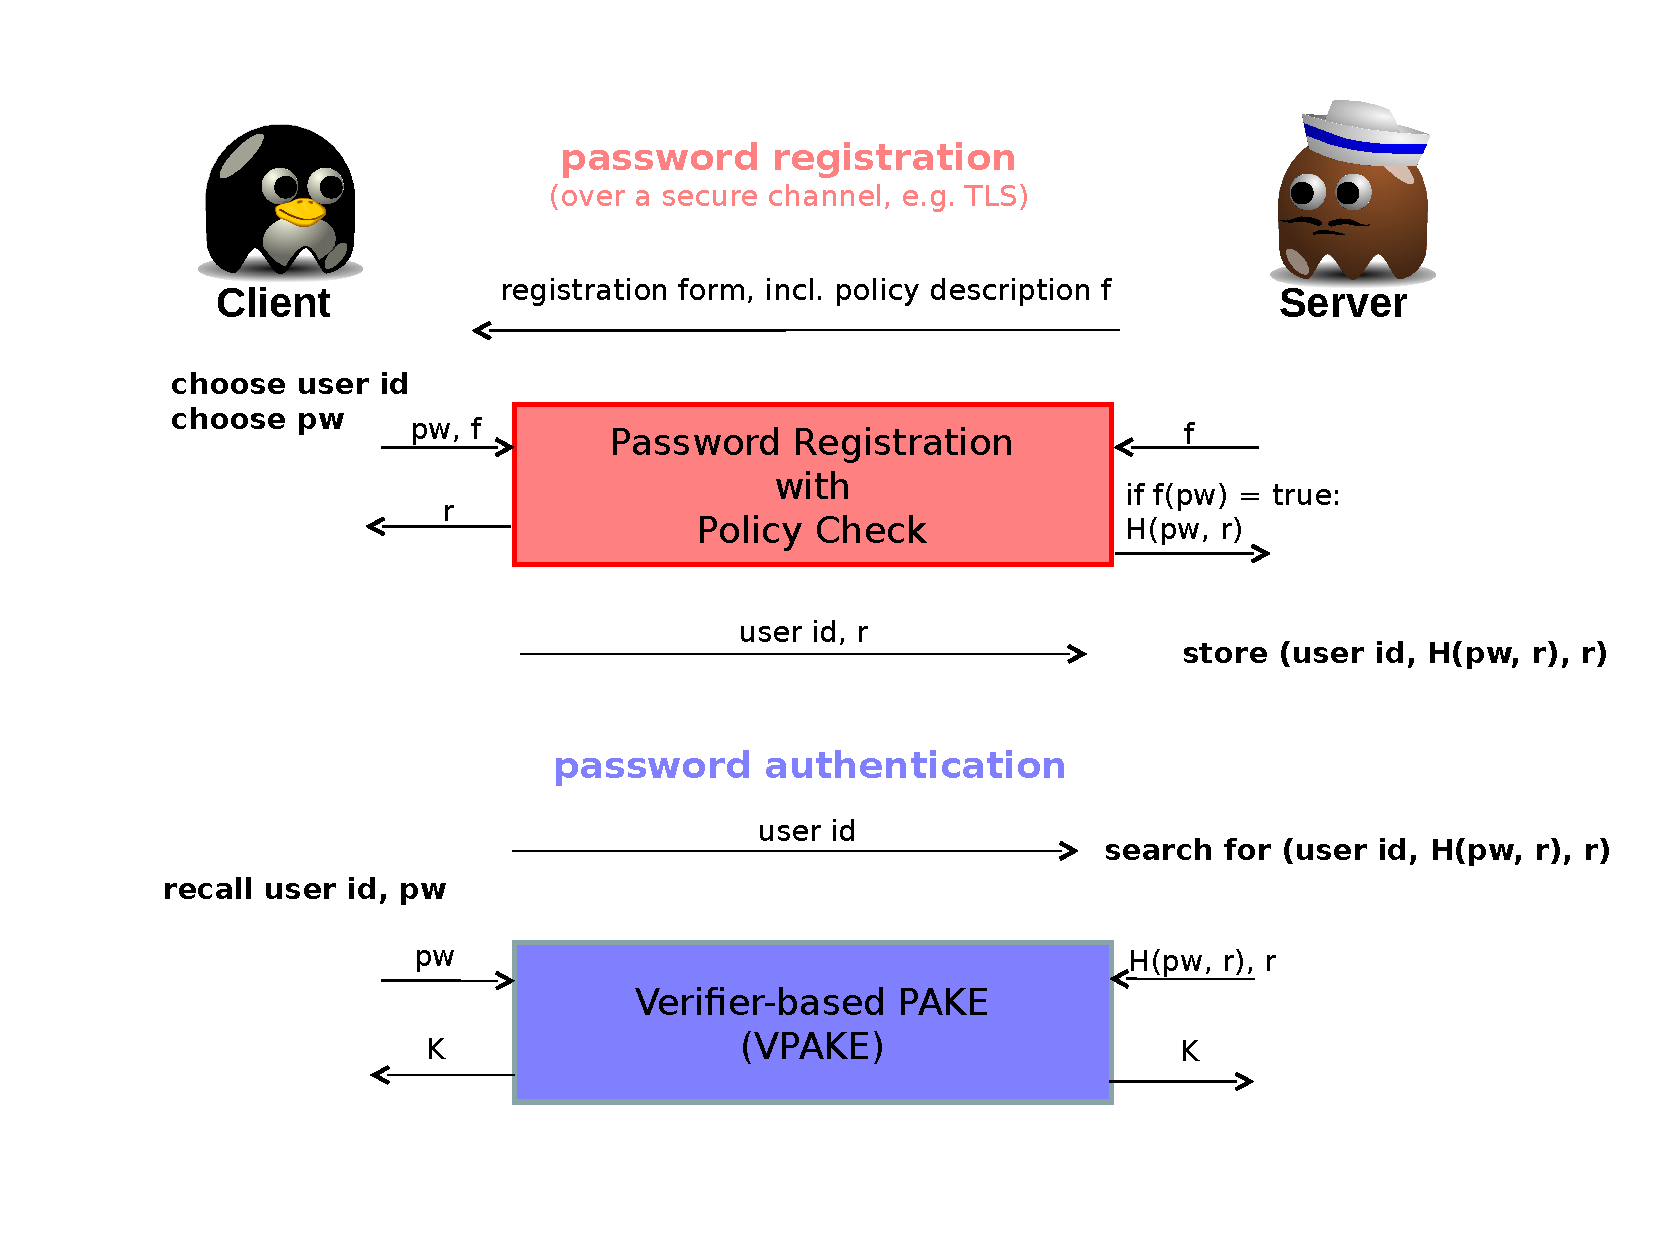
\includegraphics[width=\textwidth]{framework1.pdf}
  \end{figure}
\end{frame}

\begin{frame}{Verifier-based PAKE}{How NOT to do it}
  \begin{figure}[thbp]
  \begin{center}
  \scalebox{0.85}{\small
  \begin{tabular}{ l c l }
  \toprule
  {\bf Client} & & {\bf Server} \\
  Input: $\pwd$ & & Input: $v=(H,r)$ \\
  \midrule
  $v=(H,r)\gets \phi(\pwd, r)$ & $\xleftarrow{\makebox[2.5cm]{$r$}}$ & \\
   & $\xleftrightarrow{\makebox[2.5cm]{PAKE on $H$}}$ & \\
  \bottomrule
  \end{tabular}}
  \end{center}
  \end{figure}
  
  \begin{center}    
  \structure{This is a PAKE not a VPAKE}
  \end{center}
\end{frame}

\begin{frame}{SPHF-based VPAKE}{Framework by \cite{BenhamoudaP13}}
  \begin{figure}[t]
  \begin{center}
  \scalebox{0.7}{\small
  \begin{tabular}{ l c l }
  \toprule
  {\bf Client \Client} & & {\bf Server \Server} \\
  Input: $\pk, \Server, \pi$ & & Input: $\pk,\Client, \ver=(H_1,H_2,s_H)$ \\
  \midrule
  $\hk\gets\HKGen(L_{H})$ & & $\hk'\gets\HKGen(L_{s_H,H})$ \\
  $\hp\gets\PKGen(\hk,L_{H})$ & & $\hp'\gets\PKGen(\hk',L_{s_H,H})$ \\
  $r\rin\ZZ_p$; $\ell=(id,\bm{S},\hp)$ & & $r' \rin \ZZ_p$; $\ell'=(\bm{S},id,\hp')$ \\
  $C\gets \Enc^\ell(\pk,g_1^\pi;r)$ & & $C'\gets\Enc^{\ell'}(\pk,H_2;r')$ \\
   & $\xrightarrow{\makebox[2.5cm]{$\hp,\ C$}}$ & \\
   & $\xleftarrow{\makebox[2.5cm]{$\hp',C', H_1, s_H$}}$ & \\
  $\ell'=(\bm{S},id,\hp')$; $H_2\gets H_1^\pi h^{s_H}$ & & $\ell = (id,\bm{S},\hp)$ \\
  $K_1\gets\Hash(\hk, L_H, C')$; & & $K_1 \gets \ProjHash(\hp, L_H, C', r')$ \\
  $K_2\gets\ProjHash(\hp', L_{s_H,H}, C, \pi, r)$ & & $K_2 \gets \Hash(\hk', L_{s_H,H}, C)$\\
  $K \gets K_1 \cdot K_2$ & &  $K\gets K_1 \cdot K_2$\\
  \bottomrule
  \end{tabular}}
  \end{center}
  \end{figure}
  
  \vspace*{1em}
  \begin{center}
    \structure{Adapted to our Hash function}
    \begin{itemize}
      \item new Smooth Projective Hash Function proposed
    \end{itemize}
  \end{center}
\end{frame}

%===============================================================================
% Password Authentication Framework in the Two-Server Setting
%===============================================================================
\section{Two-Server Password Framework}%{Password Authentication Framework in the Two-Server Setting}

\begin{frame}{Table of Content}
\tableofcontents[currentsection]
\end{frame}

\begin{frame}{The Setting}
  \begin{figure}
  \begin{tikzpicture}
	  \node[state] (client) at (0,-1) [align=center]{\pgfimage[width=0.8cm]{os_tux}\\ Client $(\pwd)$};
	  \node[state] (server1) at (6,0) [align=center]{\pgfimage[width=0.8cm]{techie_sailor}\\ Server 1 $(\share_1)$};
	  \node[state] (server2) at (6,-2) [align=center]{\pgfimage[width=0.8cm]{techie_sailor}\\ Server 2 $(\share_2)$};
	  \draw[pil,<->] ($(client.west)+(1.3,0.01)$) -- (server1);
	  \draw[pil,<->] ($(client.west)+(1.3,-0.01)$) -- (server2);
  \end{tikzpicture}
  \end{figure}
\end{frame}

\begin{frame}{Two-Server Password Authentication Framework}
  \begin{figure}
  \centering
  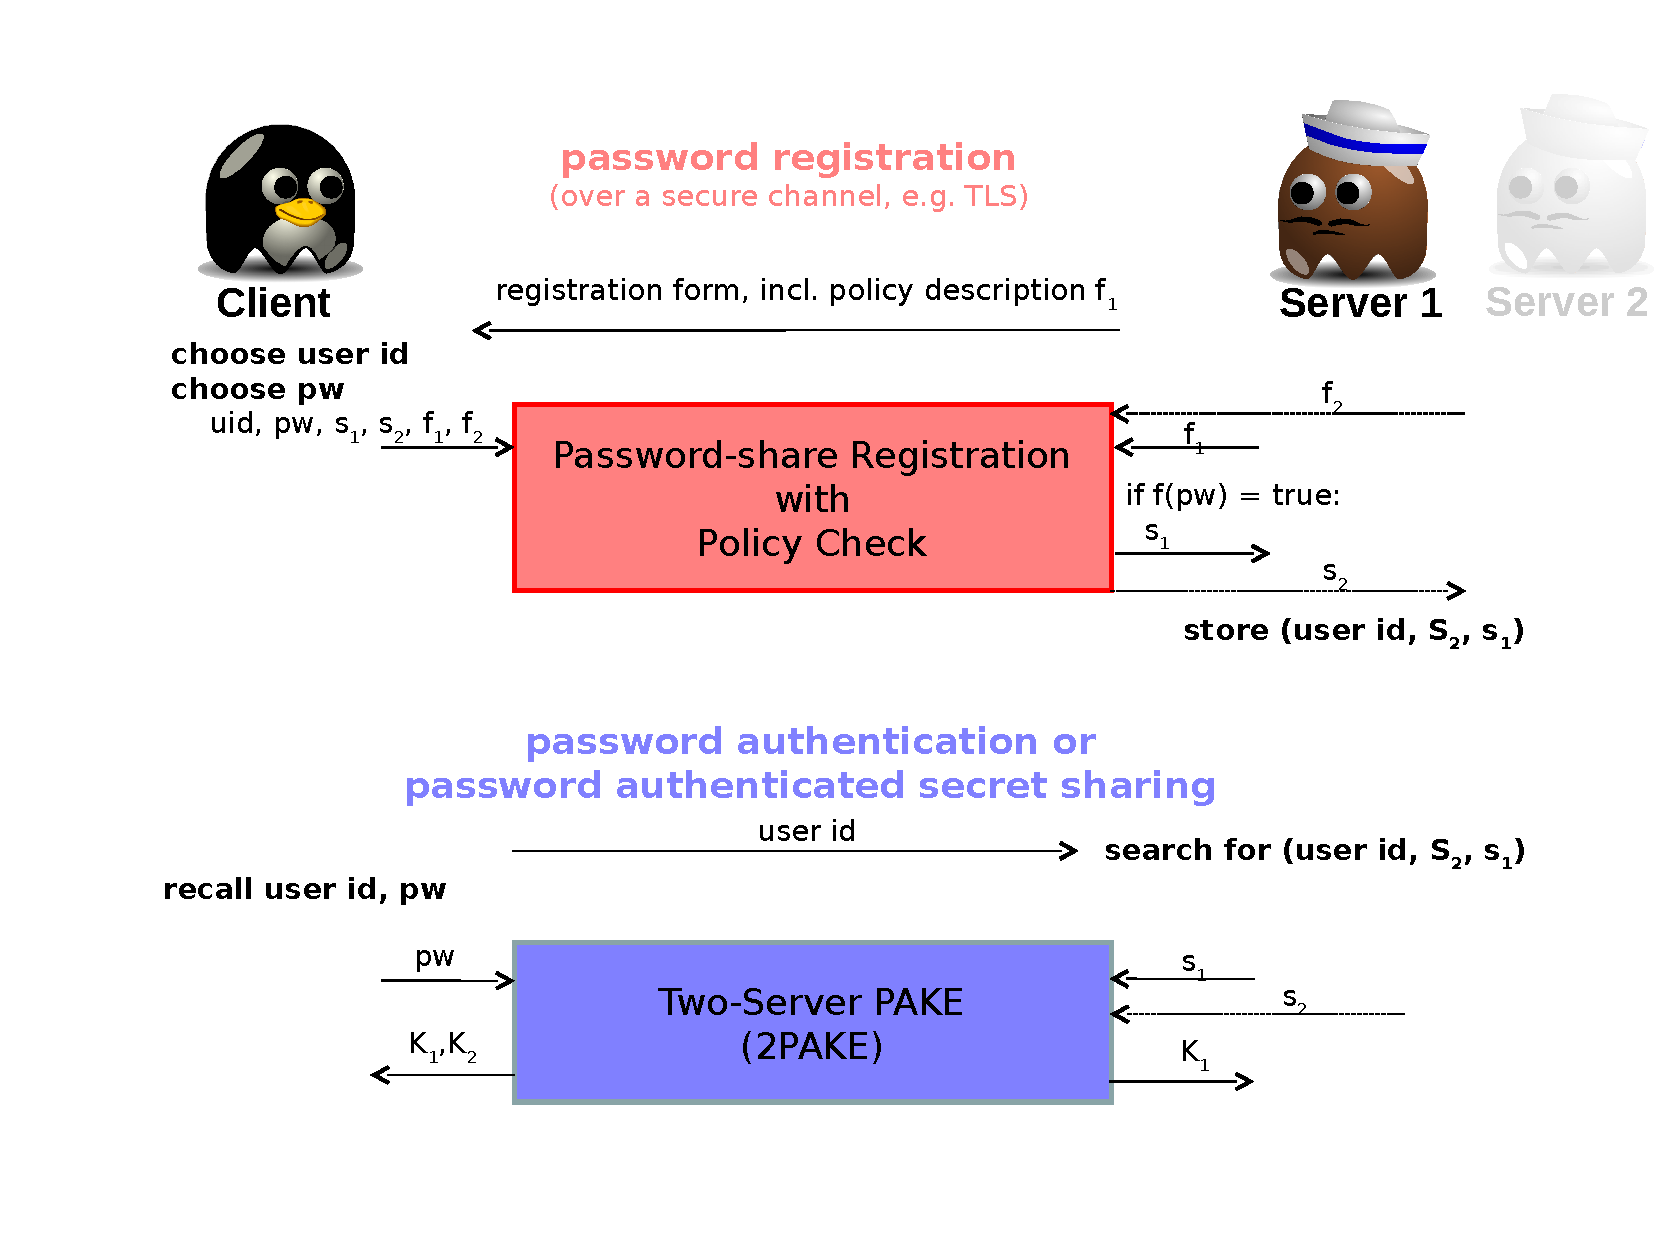
\includegraphics[width=\textwidth]{framework2.pdf}
  \end{figure}
\end{frame}

\begin{frame}{Modelling Passwords}
  \begin{itemize}
    \item Recall single-server setting:
    \begin{itemize}
      \item $f=(R,\pmin)$
      \item $\Sigma=(d,u,l,s)$
      \item $\pwd=c_1,\cdots,c_n$
    \end{itemize}
  \end{itemize}
  \vspace*{1em}
  \begin{itemize}
    \item Each server has its own $f_i$ now
    \item $f=f_1\cap f_2=(\max(R_1, R_2), \max(\pmin_1, \pmin_2))$
  \end{itemize}
\end{frame}

% \subsection{Distributed Smooth Projective Hashing \& 2-Server PAKE}

\subsection{Two-Server BPR}

\begin{frame}{Blind Password Registration for Two Servers}
  \structure{The Proof}
  \begin{align*}
    (\pwd, \share_0, \share_1):~ &\pwdint(\pwd)=\share_0 + \share_1 ~ \wedge ~ f(\pwd)=\true
  \end{align*}
\end{frame}

\begin{frame}{Security Model}
    \begin{description}
      \item[$\mathsf{Setup}(C,S_{0},S_1,\pwd')$:] \hfill \\ register a new client
      \item[$m'\gets\mathsf{Send}_C(C,S_{b},m)$:] \hfill \\ simulates active attack
      \item[$m'\gets\mathsf{Send}_S(S_b,C,m)$:] \hfill \\ simulates active attack
      \item[$m'\gets\mathsf{Send}_{SS}(S_b,S_{1-b},m)$:] \hfill \\ simulates active attack
      \item[$\mathtt{t}\gets\mathsf{Execute}(C,S_b)$:] \hfill \\ simulates passive attack
      \item[$\{(C,S_{1-b},\share_b)\}\gets\mathsf{Corrupt}(S_b)$:] \hfill \\ simulates a server breach
    \end{description}
\end{frame}

\begin{frame}{Security Model}
  \begin{definition}[Policy Compliance]\label{def:pc}
  Policy Compliance of a 2BPR protocol holds if for every PPT adversary $\cA$ with access to $\mathsf{Setup}$ and $\mathsf{Send}_C$ oracles the probability that two server instances $S_{b,i}$ and $S_{1-b,j}$ exist after $\cA$ stopped that accepted $(C,S_{1-b},\share_b)$, $(C,S_{b},\share_{1-b})$ respectively, with $f(\share_b+\share_{1-b})=\mathtt{false}$ is negligible.
  \end{definition}
\end{frame}

\begin{frame}{Security Model}
  \begin{definition}[Password Blindness]\label{def:zk}
%   The Password Blindness property of a Two-Server BPR protocol $\Pi$ holds if for every PPT adversary $A$ there exists a negligible function $\varepsilon(\cdot)$ such that
  \[ \Adv_{\Pi, \cA}^{\mathrm{PB}}=\left|\Pr[\Exp_{\Pi, \cA}^{\mathrm{PB}}=1]-\frac{1}{2}\right|\leq\varepsilon(\secpar). \]

  \structure{$\Exp_{\Pi, \cA}^{\mathrm{PB}}$}
  \begin{itemize}
    \item $(C_0, C_1, S_0, S_1,\share_0,\share_1)$ output by $\cA$ with access to $\mathsf{Setup},\mathsf{Send}_S,\mathsf{Send}_{SS}, \mathsf{Execute},\mathsf{Corrupt}$ $(\secpar,D,\{C\},\{S\})$ 
%     \item check $\share_0,\share_1\in D_{f_0\cap f_1}$, $|\share_0|=|\share_1|$, $C_0,C_1\in\{C\}$ and $S_0,S_1\in\{S\}$\\
    \item $A$ with access to $\mathsf{Setup}',\mathsf{Send}_S,\mathsf{Send}_{SS}, \mathsf{Execute},\mathsf{Corrupt}$ guesses $b'$
    \item if $S_0$ or $S_1$ is not corrupted, return $b=b'$; otherwise return $0$ 
  \end{itemize}

%   \noindent
%   $\mathsf{Setup}'$ (in contrast to $\mathsf{Setup}$) uses $\share_b$ for client $C_0$ and $\share_{1-b}$ for $C_1$ with $b\rin\{0,1\}$ instead of choosing a random password or using the provided one.
  \end{definition}
\end{frame}

\begin{frame}{A BPR Protocol}{is too long for this slide ...}
  \begin{itemize}
    \item similar to single-server BPR
    \item proofs are done over \textit{shares}
    \item additional proof that shares combine to $\pwd$
  \end{itemize}
\end{frame}

\begin{frame}
  \begin{figure}[tbhp]
  \begin{center}
  \scalebox{0.45}{
  \begin{tabular}{ l c l }
  \toprule
  {\bf Client \Client} & & \\
  Input: $\Server_0,\Server_{1}, f=f_0\cap f_1$ & &\\
  \hspace*{2.8em} $\pwd, \crs$ & & \\
  \midrule
  & \textit{I -- Client Preparation} & \\
  % \cmidrule{2-2}
  encode $\pi\gets\pwdint(\pwd)$ & & \\
  compute password shares: & & \\
  \hspace*{1em} $\share_{0}\rin\ZZ_p$, $\share_{1}=\pi-\share_{0}$ & & \\
  commit to shares: & & \\
  \hspace*{1em} $\fC_0=g^{\share_{0}}h^{r_{0}}$, $\fC_{1}=g^{\share_{1}}h^{r_{1}}$ & & \\
  \hspace*{1em} $\fD_0=\fC_0g^{\share_{1}}$, $\fD_{1}=\fC_{1}g^{\share_{0}}$ & & \\
  \midrule
  {\bf Client \Client} & & {\bf Server $\Server_b$} \\
  Input: $\Server_0,\Server_{1}, f=f_0\cap f_1$ & & Input: $\Client,\Server_{1-b}$ \\
  \hspace*{2.8em} $\pwd, \crs$ & & \hspace*{2.8em} $f=f_0\cap f_1, \crs$ \\
  \midrule
  & \textit{II -- Password Registration} & \\
  % \cmidrule{2-2}
  commit to all characters: & & \\
  \hspace*{1em} $C_i=g^{\pi_i}h^{r_i};~ C'_i=C_ih^{r'_i}$ & & \\
  shuffle $\bm C'$ s.t. $C'_i=C_{\phi(i)}h^{r'_{\phi(i)}}$ & & \\
  with permutation $\phi$ & & \\
  for $c_i\in\pwd$ identify set $\omega_{\phi(i)}$ & & \\
  execute \PoC, \PoM, \PoS & & \\
   & $\xrightarrow{\makebox[4cm]{$\Comm_{\PoM}, \Comm_{\PoC}, \Comm_{\PoS}$}}$ & \\
   & $\xleftarrow{\makebox[4cm]{$\Ch_{\PoM}, \Ch_{\PoC}, \Ch_{\PoS}$}}$ & choose challenges\\
   & $\xrightarrow{\makebox[4cm]{$\Res_{\PoM}, \Res_{\PoC}, \Res_{\PoS}$}}$ & Proceed if\\
   & & $|\bm C|=|\bm C'| \geq \pmin, \PoM$\\
   & & $\PoC$ and $\PoS$ all holds\\
  \midrule
  {\bf Server $\Server_0$} & & {\bf Server $\Server_1$} \\
  Input: $\Client, \Server_{1}$ & & Input: $\Client,\Server_{0}$ \\
  \hspace*{2.8em} $f=f_0\cap f_1, \crs$ & & \hspace*{2.8em} $f=f_0\cap f_1, \crs$ \\
  \midrule
  & \textit{III -- Share Verification} & \\
  % \cmidrule{2-2}
  $\fD'_{1}=\fC_{1}g^{\share_{0}}$ & $\xrightarrow{\makebox[4cm]{$\fD'_{1}$}}$ & $\fD'_{0}=\fC_{0}g^{\share_{1}}$ \\
  If $\fD'_0=\fD_0$ & $\xleftarrow{\makebox[4cm]{$\fD'_{0}$}}$ & If $\fD'_{1}=\fD_{1}$ \\
  \hspace*{1em} store $(\Client,\Server_{1},\share_{0})$ & & \hspace*{1em} store $(\Client,\Server_{0},\share_{1})$ \\
  \bottomrule
  \end{tabular}}
  \end{center}
  \end{figure}
\end{frame}

% \subsection{Distributed Smooth Projective Hashing}
\subsection{DSPHF \& A 2-Server PAKE Framework}

\begin{frame}{Smooth Projective Hashing}

\begin{dynblock}
\opaqueblock<1>{\hspace*{1em}
Let $L_x$ denote a language such that $C\in L_x$ if there exists a witness $w$ proving so.
\begin{description}
	\item[$\HKGen(L_x)$]\hfill\\ generates a hashing key \hk for language $L_x$.
	\item[$\PKGen(\hk,L_x,C)$]\hfill\\ derives the projection key \hp, possibly depending on $C$.
	\item[$\Hash(\hk,L_x,C)$] \hfill\\ outputs the hash value $h$.
	\item[$\PHash(\hp,L_x,C,w)$] \hfill\\ returns the hash value $h$.
\end{description}
}
\invblock<2->

\opaqueblock<2>{\hspace*{1em}
	\begin{description}
		\item[Correctness]\hfill\\ If $C\in L_x$, with $w$ proving so, then $\mathsf{Hash}(\hk,L_x,C)=\mathsf{PHash}(\hp,L_x,C,w)$.
		\item[Smoothness]\hfill\\ If $C\not\in L_x$, the hash value $h$ is statistically indistinguishable from a random element.
		\item[Pseudorandomness]\hfill\\ If $C\in L_x$, the hash value $h$ is indistinguishable from a random element.
	\end{description}
}
\end{dynblock}

\end{frame}

% \begin{frame}{PAKE from SPHF}
% \begin{figure}
% \centering
% \begin{tikzpicture}
% 	\node[state, align=center] (client) at (0,1) {\pgfimage[width=0.8cm]{os_tux}\\ $\pwd$};
% 	
% 	\node[state, align=left] at (0,-1) {$k_h\gets\mathsf{KGen_H}(L_x)$\\  $k_p\gets\mathsf{KGen_P}(k_h,L_x)$\\  $C\gets\mathsf{Enc}_\pk(\pwd;r)$};
% 	\node[state] (client1) at (2,-1){};
% 	
% 	\node[state] (client2) at (2,-2){};	
% 	\node[state, align=left] at (0,-3) {$k\gets\mathsf{Hash}(k_h,L_x,C')$\\$\cdot\mathsf{PHash}(k'_p,L_x,C,r)$};
% 	
% 	\node[state, align=center] (server) at (6,1) {\pgfimage[width=0.8cm]{techie_sailor}\\ $\pwd$};
% 	
% 	\node[state, align=right] at (6,-1) {$k'_h\gets\mathsf{KGen_H}(L_x)$\\  $k'_p\gets\mathsf{KGen_P}(k_h,L_x)$\\  $C'\gets\mathsf{Enc}_\pk(\pwd;r')$};
% 	\node[state] (server1) at (4,-1) {};
% 	
% 	\node[state] (server2) at (4,-2) {};
% 	\node[state, align=right] at (6,-3) {$k\gets\mathsf{Hash}(k'_h,L_x,C)$\\$\cdot\mathsf{PHash}(k_p,L_x,C',r')$};
% 	
% 	%\node[state, align=center] at (6,-3) {$K\gets H(A,B,X',Y',K_B,\pwd)$};
% 	
% 	\draw[pil] (client1) -- node[above] {$C,k_p$} (server1);
% 	\draw[pil] (server2) -- node[above] {$C',k'_p$} (client2);
% \end{tikzpicture}
% \label{fig:eke}
% \end{figure}
% \end{frame}

\begin{frame}{Extended Smooth Projective Hashing 1/2}

%Languages of ciphertexts: $C\gets\mathsf{Enc}_{\pk}(x)$
%2-Server PAKE between \begin{center} Client$(\pwd)$, Server$_1(\share_1)$, Server$_2(\share_2)$\end{center}

\begin{figure}
\begin{tikzpicture}
	\node[state] (client) at (0,-1) [align=center]{\pgfimage[width=0.8cm]{os_tux}\\ Client $(\pwd)$};
	\node[state] (server1) at (6,0) [align=center]{\pgfimage[width=0.8cm]{techie_sailor}\\ Server 1 $(\share_1)$};
	\node[state] (server2) at (6,-2) [align=center]{\pgfimage[width=0.8cm]{techie_sailor}\\ Server 2 $(\share_2)$};
	\draw[pil] ($(client.west)+(1.2,0)$) -- (server1);
	\draw[pil] ($(client.west)+(1.2,0)$) -- (server2);
\end{tikzpicture}
\end{figure}

\setbeamercolor{uppercol}{fg=white,bg=blue!40}%
\setbeamercolor{lowercol}{fg=black,bg=blue!20}%
\begin{beamerboxesrounded}[upper=uppercol,lower=lowercol,shadow=true]{\centering Idea}
	Encrypt $\pwd$, $\share_1$ and $\share_2$ $\rightarrow$ Use extended SPHF to compute keys
\end{beamerboxesrounded}

\end{frame}

\begin{frame}{Extended Smooth Projective Hashing 2/2}

\begin{description}
	\item[$\mathsf{KGen_H}(L_x)$]\hfill\\ generates a hashing key $k_h$ for language $L_x$.
	\item[$\mathsf{KGen_P}(k_h,L_x)$]\hfill\\ derives the projection key $k_h$.
	\item[$\mathsf{Hash}_x (k_{h,0},L_x,C_1,C_2)$]\hfill\\ outputs the hash value $h_x$.
	\item[$\mathsf{PHash}_x (k_{p,0},L_x,C_1,C_2,w_1,w_2)$]\hfill\\ returns the hash value $h_x$.
	\item[$\mathsf{Hash}_0(k_{h,1},k_{h,2},L_x,C_0)$]\hfill\\ outputs the hash value $h_0$.
	\item[$\mathsf{PHash}_0(k_{p,1},k_{p,2},L_x,C_0,w_0)$]\hfill\\ returns the hash value $h_0$.
\end{description}

\end{frame}

\begin{frame}{Distributed (Extended) Smooth Projective Hashing}{DSPHF}

\structure{$\mathsf{PHash}_x^D$} between $S_1$ and $S_2$.\\
	\hspace*{2em} Each $S_i$ performs $\mathsf{PHash}_x^D$ on input $$(k_{p,0},C_1,C_2,w_i)$$\hspace*{2em} such that $S_1$ eventually holds $h_x$.
	
	\vspace*{2em}
\structure{$\mathsf{Hash}_0^D$} between $S_1$ and $S_2$.\\
	\hspace*{2em} Each $S_i$ performs $\mathsf{Hash}_0^D$ on input $$(\share_i,k_{h,i}, C_0)$$\hspace*{2em} such that $S_1$ eventually holds $h_0$.

\end{frame}

\begin{frame}{2-Server PAKE from DSPHF}

		\begin{figure}
		\begin{tikzpicture}
			\node[state] (client) at (0,-2) [align=center]{\pgfimage[width=0.8cm]{os_tux}\\ Client $(\pwd)$\\\hspace*{0cm}\\};
			\node[state] (server1) at (6,0) [align=center]{\pgfimage[width=0.8cm]{techie_sailor}\\ Server 1 $(\share_1)$};
			\node[state] (server2) at (6,-4) [align=center]{\pgfimage[width=0.8cm]{techie_sailor}\\ Server 2 $(\share_2)$};
	
			\draw[pil,->] ($(client.west)+(2,0.2)$) -| node[above,anchor=center,xshift=-1.5cm,yshift=-0.8cm]{$k_p,C$} (server1);
			\draw[pil,->] ($(client.west)+(2,-0.2)$) -| node[below,anchor=center,xshift=-1.5cm,yshift=0.8cm]{$k_p,C$} (server2);
			\draw[pil,<-] ($(client.west)+(1.2,0)$) -- node[above,anchor=center]{$k_{p,1},C_1$} (server1);
			\draw[pil,<-] ($(client.west)+(1.2,0)$) -- node[below,anchor=center]{$k_{p,2},C_2$} (server2);
		\end{tikzpicture}
		\end{figure}

\end{frame}

\begin{frame}{2-Server PAKE from DSPHF}

		\begin{figure}
		\begin{tikzpicture}
			\node[state] (client) at (0,-2) [align=center]{\pgfimage[width=0.8cm]{os_tux}\\ Client $(\pwd)$\\ $\PHash_0\cdot\Hash_x$\\ $\rightarrow \sk$};
			\node[state] (server1) at (6,0) [align=center]{\pgfimage[width=0.8cm]{techie_sailor}\\ Server 1 $(\share_1)$\\ $h_x\cdot h_0\rightarrow \sk$};
			\node[state] (server2) at (6,-4) [align=center]{\pgfimage[width=0.8cm]{techie_sailor}\\ Server 2 $(\share_2)$};
	
			\draw[pil,<->] (server1) -- node[anchor=center,xshift=-0.1cm]{$\PHash_x^D$~~~~$\Hash_0^D$} (server2);
%			\draw[pil,<-] ($(client.west)+(1.2,0)$) -- node[below,anchor=center]{$k_{p,2},C_2$} (server2);
		\end{tikzpicture}
		\end{figure}

\end{frame}

\subsection{UC 2Server PAKE}

\begin{frame}{UC Security for 2Server PAKE}
  \structure{Trapdoor Distributed Smooth Projective Hash Function}
  \begin{itemize}
    \item extending D-SPHF further
    \item trapdoor SPHF introduced by \cite{Benhamouda2013}
    \item necessary for \emph{efficient} UC-secure protocol
    \item $\mathsf{THash}$ can compute hash without hashing key, uses trapdoor instead
    \item $\mathsf{VerKp}$ verifies that $k_p$ is a valid projection key
    \item Using previous 2PAKE framework with TD-SPHF yields UC-secure 2PAKE
  \end{itemize}
\end{frame}

\begin{frame}{UC 2PAKE Funcitonality}{Overview}
  \begin{description}

    \item[KEX Init$_\Client$:] \hfill\\ initialise client
    \item[KEX Init$_\Server$:] \hfill\\ initialise server
    \item[TestPwd:] \hfill\\ check if a password is used by a client
    \item[Failed:] \hfill\\ mark protocol run as failed
	  \item[NewKey:] \hfill\\ compute a new session key as result
	
  \end{description}
\end{frame}

\begin{frame}{UC 2PAKE Funcitonality}{KEX Init$_\Client$}
    Upon input $(\KEXinit, \sid, \qid, \pwd)$ from client \Client, check that \sid is $(\Client, \Server_1, \Server_2)$ and that \qid is unique (entries $(\KEX, \sid, \qid, \Server_{1}, \share_{1})$ or $(\KEX, \sid, \qid, \Server_{2}, \share_{2})$ may exist) and send $(\KEX, \sid, \qid, C)$ to \SIM.
        If this is a valid request, create a \emph{fresh} record $(\KEX, \sid, \qid, \Client, \pwd)$.
\end{frame}

\begin{frame}{UC 2PAKE Funcitonality}{KEX Init$_\Server$}
  
Upon input $(\KEXinit, \sid, \qid, \share_b)$ from server $\Server_b$, $b\in\{1,2\}$, check that \sid is $(\Client, \Server_1, \Server_2)$ and that \qid is unique (entries $(\KEX, \sid, \qid, \Client, \pwd)$ or $(\KEX, \sid, \qid, \Server_{3-b}, \share_{3-b})$ may exist) and send $(\KEX, \sid, \qid, \Server_b)$ to \SIM.
        If this is a valid request, create a fresh record $(\KEX, \sid, \qid, \Server_b, \share_b)$.
\end{frame}

\begin{frame}{UC 2PAKE Funcitonality}{TestPwd}  
    Upon input $(\TP, \sid, \qid, \pwd')$ from \SIM check that a fresh record $(\KEX, \sid, \qid, \Client, \pwd)$ exists. 
        If this is the case, mark $(\KEX, \sid, \qid, \Server_1, \share_1)$ as \compromised and reply with ``correct guess'' if $\pwd=\pwd'$, and mark it as \interrupted and reply with ``wrong guess'' if $\pwd\not=\pwd'$.
\end{frame}
      
\begin{frame}{UC 2PAKE Funcitonality}{Failed}
  Upon input $(\FA, \sid, \qid)$ from \SIM check that records $(\KEX, \sid, \qid, \Client, \pwd)$ and $(\KEX, \sid, \qid, \Server_1, \share_1)$ exist that are not marked \completed. 
        If this is the case, mark both as \failed.
\end{frame}
  
\begin{frame}{UC 2PAKE Funcitonality}{NewKey}
	  Upon input $(\NK, \sid,\qid, P, \sk')$ from \SIM with $P\in\{\Client,\Server_1\}$, check that a respective $(\KEX, \sid, \qid, \Client, \pwd)$ or $(\KEX, \sid, \qid, S, \share_1)$ record exists, $\sid=(\Client, \Server_1, \Server_2)$, $|\sk'|=\secpar$, then: %and the session is not marked for $P$ yet,
	  \begin{itemize}
		  \item If the session is \compromised, or either \Client or $\Server_1$ and $\Server_2$ are corrupted, then output $(\NK, \sid,\qid,\sk')$ to $P$; else
		
		  \item if the session is \emph{fresh} and a key $\sk$ was sent to $P'$ with $\sid=(P, P', \Server_2)$ or $\sid=(P', P, \Server_2)$ while $(\KEX, \sid, \qid, P', \cdot)$ was fresh, then output $(\NK, \sid, \qid, \sk)$ to $P$.
		
		  \item In any other case, pick a new random key $\sk$ of length $\secpar$, and send $(\NK, \sid, \qid, \sk)$ to $P$.
	  \end{itemize}
	  In any case, mark \qid as \completed for $P$.
\end{frame}  

%===============================================================================
% Future Work
%===============================================================================
\section{Summary}

% \begin{frame}{Table of Content}
% \tableofcontents[currentsection]
% \end{frame}

% \subsection{Summary}

\begin{frame}{Summary of Contributions}

\begin{itemize}\itemsep1em
	\item Modelling of Password Policies
	\item Blind Password Registration protocols and model (single and two-server setting)
	\item (Trapdoor) Distributed SPHF
	\item 2-Server PAKE framework
	\item 2-Server UC PAKE security
\end{itemize}

\end{frame}

% \subsection{Future Work}
%
% \begin{frame}{Future Work}
%
% 	\structure{Work in Progress}
% 	\begin{itemize}
% 		\item Secure Mobile Logins
% 		\item Zero Knowledge Password Policy Checker
% 	\end{itemize}
%
% 	\vspace*{2em}
% 	\structure{Planned Projects}
% 	\begin{itemize}
% 		\item 2-Server PAKE in UC
% 		\item 2-Server password authenticated secret sharing in the password-only model
% 		\item Trying to understand the forward-secrecy in game-based PAKE
% 	\end{itemize}
%
% \end{frame}

%===============================================================================
% Appendix
%===============================================================================

\newcommand{\beginbackup}{
   \newcounter{framenumbervorappendix}
   \setcounter{framenumbervorappendix}{\value{framenumber}}
}
\newcommand{\backupend}{
   \addtocounter{framenumbervorappendix}{-\value{framenumber}}
   \addtocounter{framenumber}{\value{framenumbervorappendix}} 
}

\beginbackup
\appendix
\section<presentation>*{\appendixname}
\subsection<presentation>*{References}

\begin{frame}[allowframebreaks]
  \frametitle<presentation>{References}
  \bibliographystyle{abbrvnat}
  \bibliography{references}
\end{frame}
\backupend

\end{document}
